\documentclass[12pt]{article}

\usepackage[a4paper]{geometry}
\usepackage[absolute,overlay]{textpos}
\usepackage{graphicx}
\usepackage{tabularx}
\usepackage{hyperref}
\usepackage{adjustbox}
\usepackage{ucs}
\usepackage[utf8]{inputenc}
\usepackage{titling}
%\usepackage{textcomp}
\PrerenderUnicode{ěščřžýáíéĚŠČŘŽÝÁÍÉďťňĎŤŇůúÚóÓ}

\usepackage[czech]{babel}

\usepackage[czech]{babel}
\usepackage[T1]{fontenc}
\usepackage{lmodern}
\usepackage[version=4]{mhchem} 

\newcommand{\subtitle}[1]{%
	\posttitle{%
		\par\end{center}
	\begin{center}\large#1\end{center}
	\vskip0.5em}%
}

\begin{document}
\title{C6250 Metody chemického výzkumu - praktikum}

\subtitle{Infračervená, Ramanova a NMR spektroskopie}

\author % (optional, for multiple authors)
{Zdeněk Moravec, hugo@chemi.muni.cz}

\date{}

\maketitle

\pagebreak

\section{Průběh cvičení}
\href{https://docs.google.com/spreadsheets/d/1izDYdwXzwPtQ4eQQNLqr0kmJblElyLACq6_Hy9QPg7c/edit?usp=sharing}{\emph{Kliknutím na tento text se dostanete do formuláře, kde si můžete zvolit datum konání cvičení.}}
\\
\rule{\textwidth}{2pt}
\\
	Cvičení probíhá v laboratořích A12/112, A12/215 a A8/1S12. Doba cvičení je 4-5 hodin.

	\begin{enumerate}
	\item Krátký úvod k IR spektroskopii \textit{(A12/112 nebo A12/215)}
	\item Spuštění spektrometrů, stanovení vlhkosti uvnitř přístroje
	\item Měření IR spekter vzorků v KBr tabletách a metodou ATR
	\item Interpretace IR spekter
	\item Měření Ramanových spekter \textit{(A12/215)}
	\item Interpretace Ramanových spekter 
	\item Krátký úvod k NMR spektroskopii \textit{(A8/1S16)}
	\item Měření NMR spekter na benchtop NMR spektrometrech Magritek 60~MHz a Bruker Avance III 300~MHz
	\item Interpretace NMR spekter
	\end{enumerate}

\subsection{Protokol}

	\begin{enumerate}
	\item Hlavička (Jméno, datum konání cvičení)
	\item Princip
	\item Postup
	\item Spektra (naměřená spektra studenti dostanou v textovém formátu)
	\item Interpretace spekter
	\item Závěr
	\end{enumerate}
	\hrule
	\begin{itemize}
		\item Protokol zašlete na adresu hugo@chemi.muni.cz do dvou týdnů ode dne konání cvičení.
	\end{itemize}

\section{Infračervená spektroskopie}

\subsection{Stanovení vlhkosti uvnitř IR spektrometru}
Hodnota vlhkosti uvnitř spektrometru je důležitá, protože optika je citlivá na stopy vlhkosti. Pro stanovení vlhkosti nastavíme spektrometr následujícím způsobem:

\begin{tabular}{|c|l|}
	\hline
	Počet skenů (background) & 16 \\\hline
	Počet skenů (vzorek) & 1 \\\hline
	Rozlišení & 2~cm$^{-1}$ \\\hline
\end{tabular}

Po změření uložíme pozadí a odečteme hodnotu maximální intenzity (I$_{MAX}$) a hodnotu intenzity pásu 1559~cm$^{-1}$ (I$_{1559}$). Vlhkost pak vypočítáme:
\\
\\
$M_{REL} = (1 - \frac{I_{1559}}{I_{MAX}}) \cdot 100 \%$

\begin{center}
	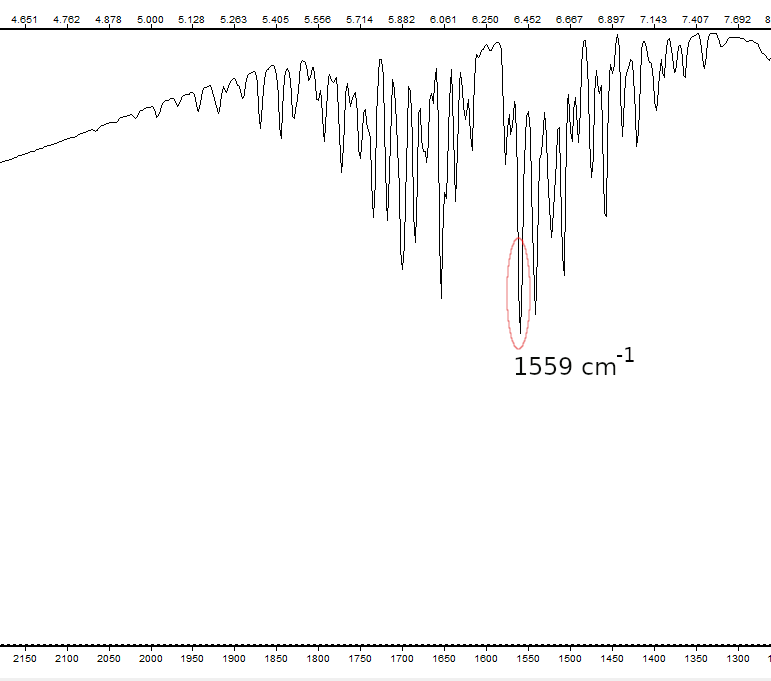
\includegraphics[keepaspectratio,height=13cm]{img/moisture.png}
\end{center}

\subsection{Měření IR spekter vzorků v suspenzi v KBr tabletách}
	1-3 mg vzorku smícháme s cca 300 mg KBr a směs rozetřeme v~achátové třecí misce. Získaný prášek nasypeme do lisovací matrice a lisujeme pod tlakem 7-9 tun po dobu cca 1 minuty.
\begin{center}
	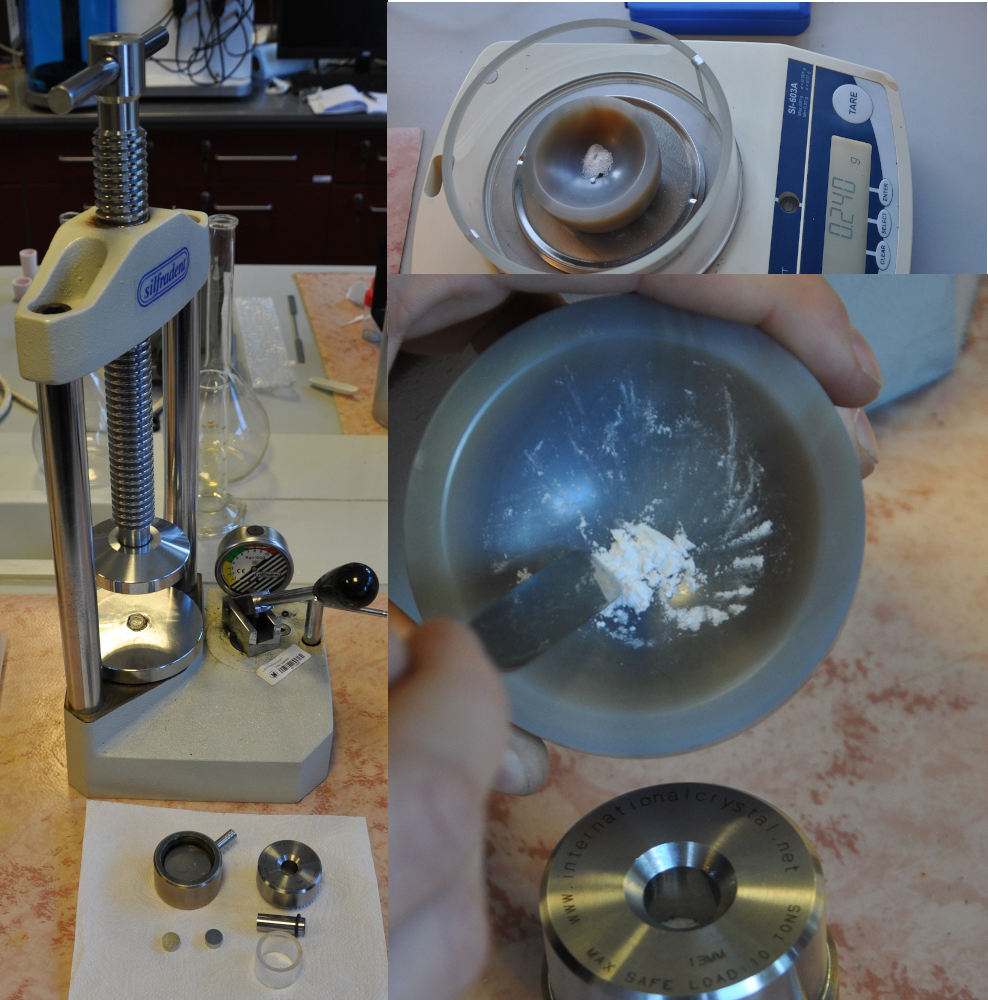
\includegraphics[keepaspectratio,height=15cm]{img/KBr.png}
\end{center}
\newpage

\subsection{Měření IR spekter vzorků metodou ATR}
Vzorek nasypeme na krystal diamantu, přitlačíme hrotem a změříme spektrum. Vzorky není potřeba žádným způsobem upravovat.

\begin{center}
	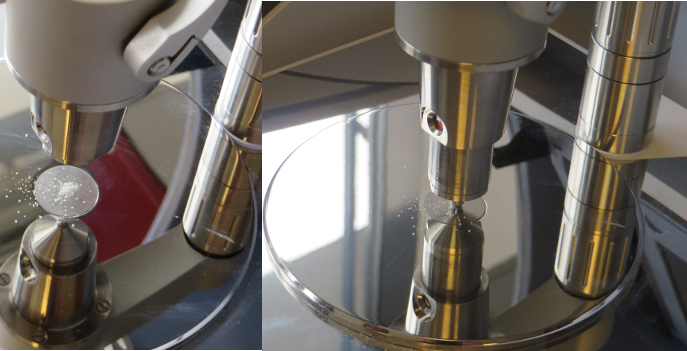
\includegraphics[keepaspectratio,width=10cm]{img/atr.png}
\end{center}

\subsection{Vyhodnocení}

Studenti dostanu naměřená IR spektra v textovém formátu, úkolem bude vytvořit grafický záznam spektra a přiřadit nejintenzivnější pásy vibracím vazeb v molekule vzorku.

%%%%%%%%%%%%%%%%%%%%%%%%%%%%%%%%%%%%%%%%%%
\newpage
\section{Ramanova spektroskopie}

Vzorek naplníme do Ramanských kapilár - kapiláry ze speciálního skla o průměru 0,8~mm, kapiláru je nutné naplnit do výšky alespoň 5~mm. Půl hodiny před měřením je nutné začít chladit detektor spektrometru kapalným dusíkem.

\begin{center}
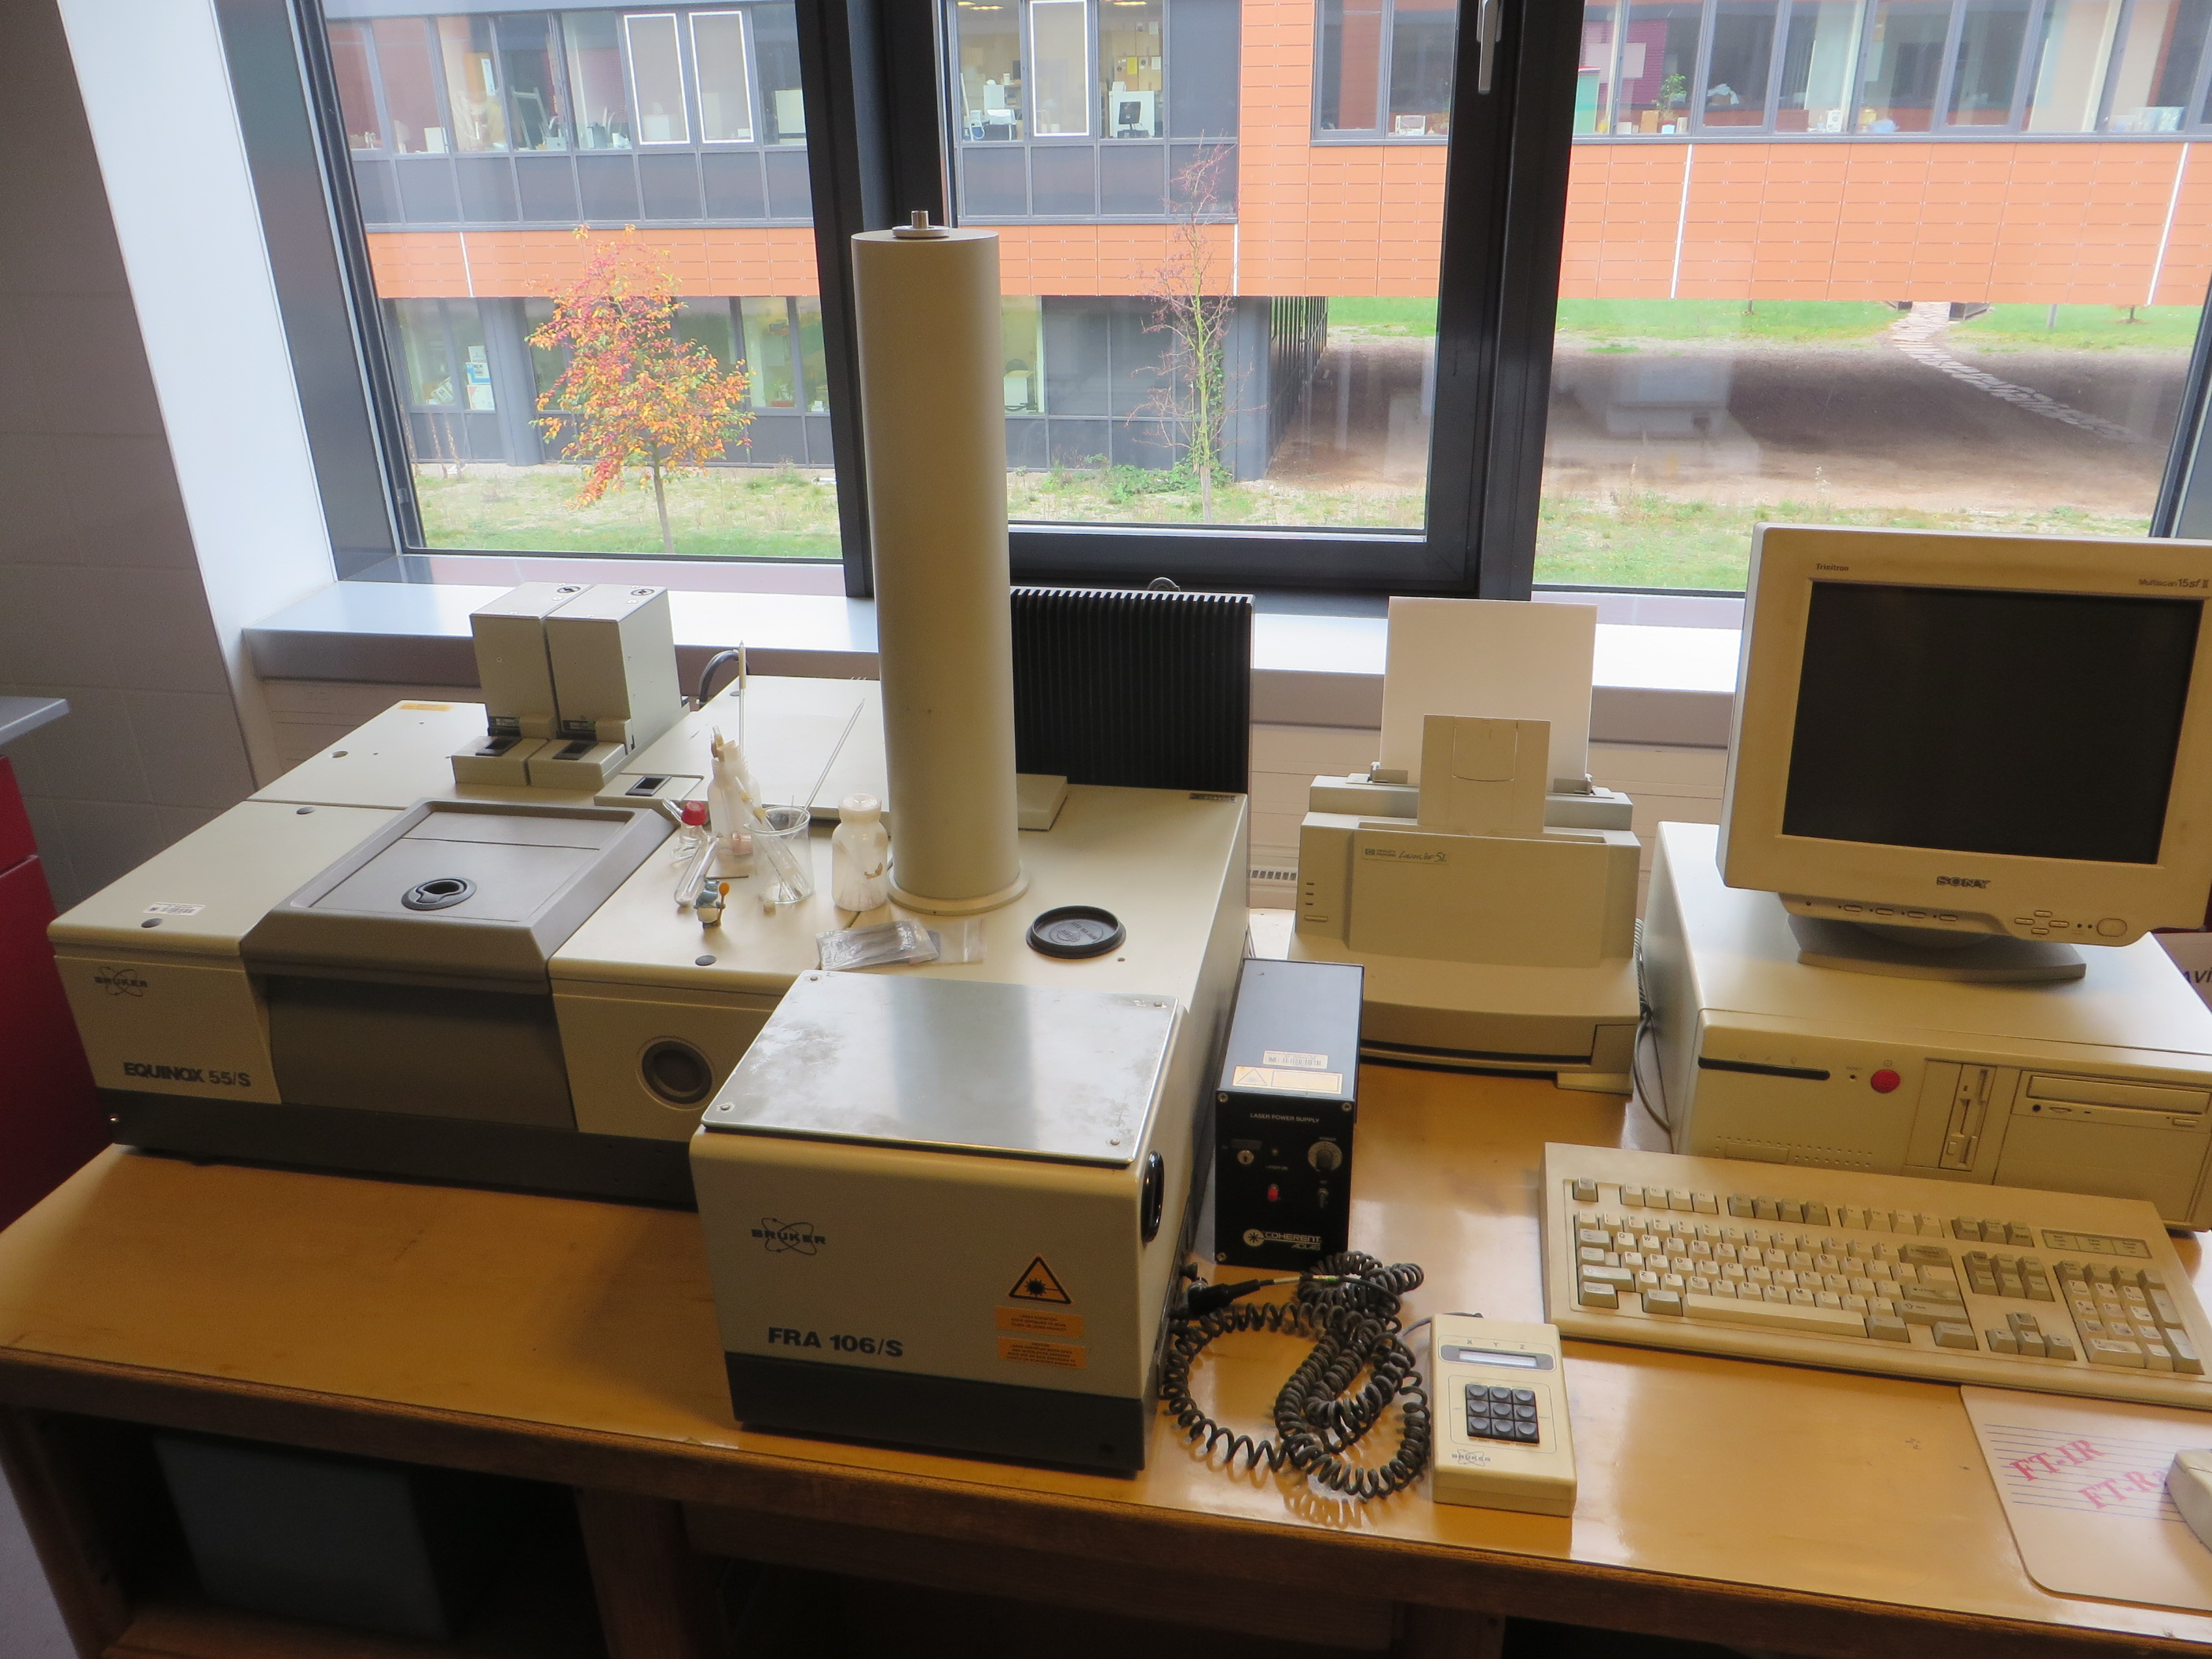
\includegraphics[keepaspectratio,width=\textwidth]{img/equinox.jpg}
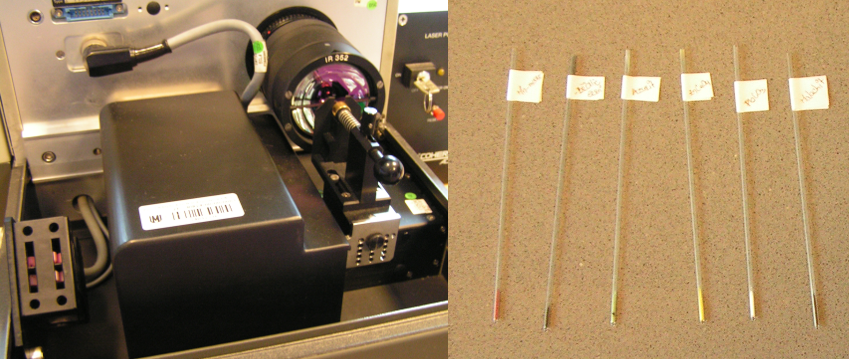
\includegraphics[keepaspectratio,width=\textwidth]{img/raman.png}
\end{center}
%%%%%%%%%%%%%%%%%%%%%%%%%%%%%%%%%%%%%%%%%%
\newpage
\section{Spektroskopie nukleární magnetické rezonance}
	\begin{itemize}
	\item Měření bude probíhat na spektrometrech Magritek 60~MHz a Bruker Avance III 300~MHz.
	\item Cílem měření bude demonstrace vlivu síly magnetického pole na rozlišení NMR spektra a ukázka interpretace 1D a 2D spekter jednoduchých organických sloučenin.
	\end{itemize}
	\begin{center}
		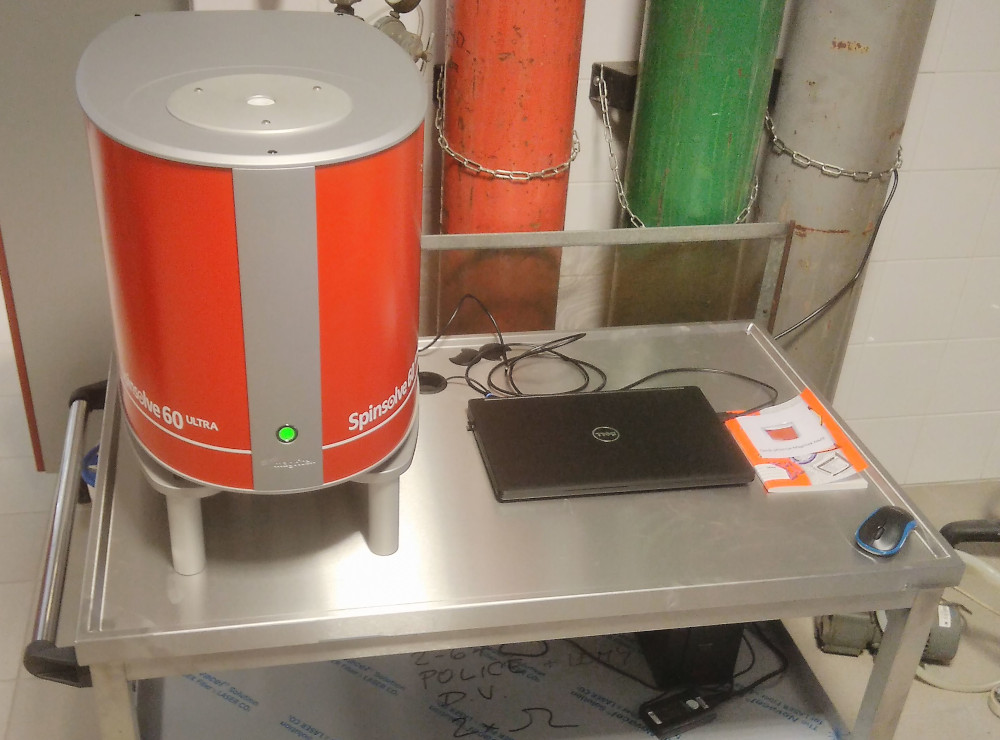
\includegraphics[keepaspectratio,height=6cm]{img/Magritek.jpg}
		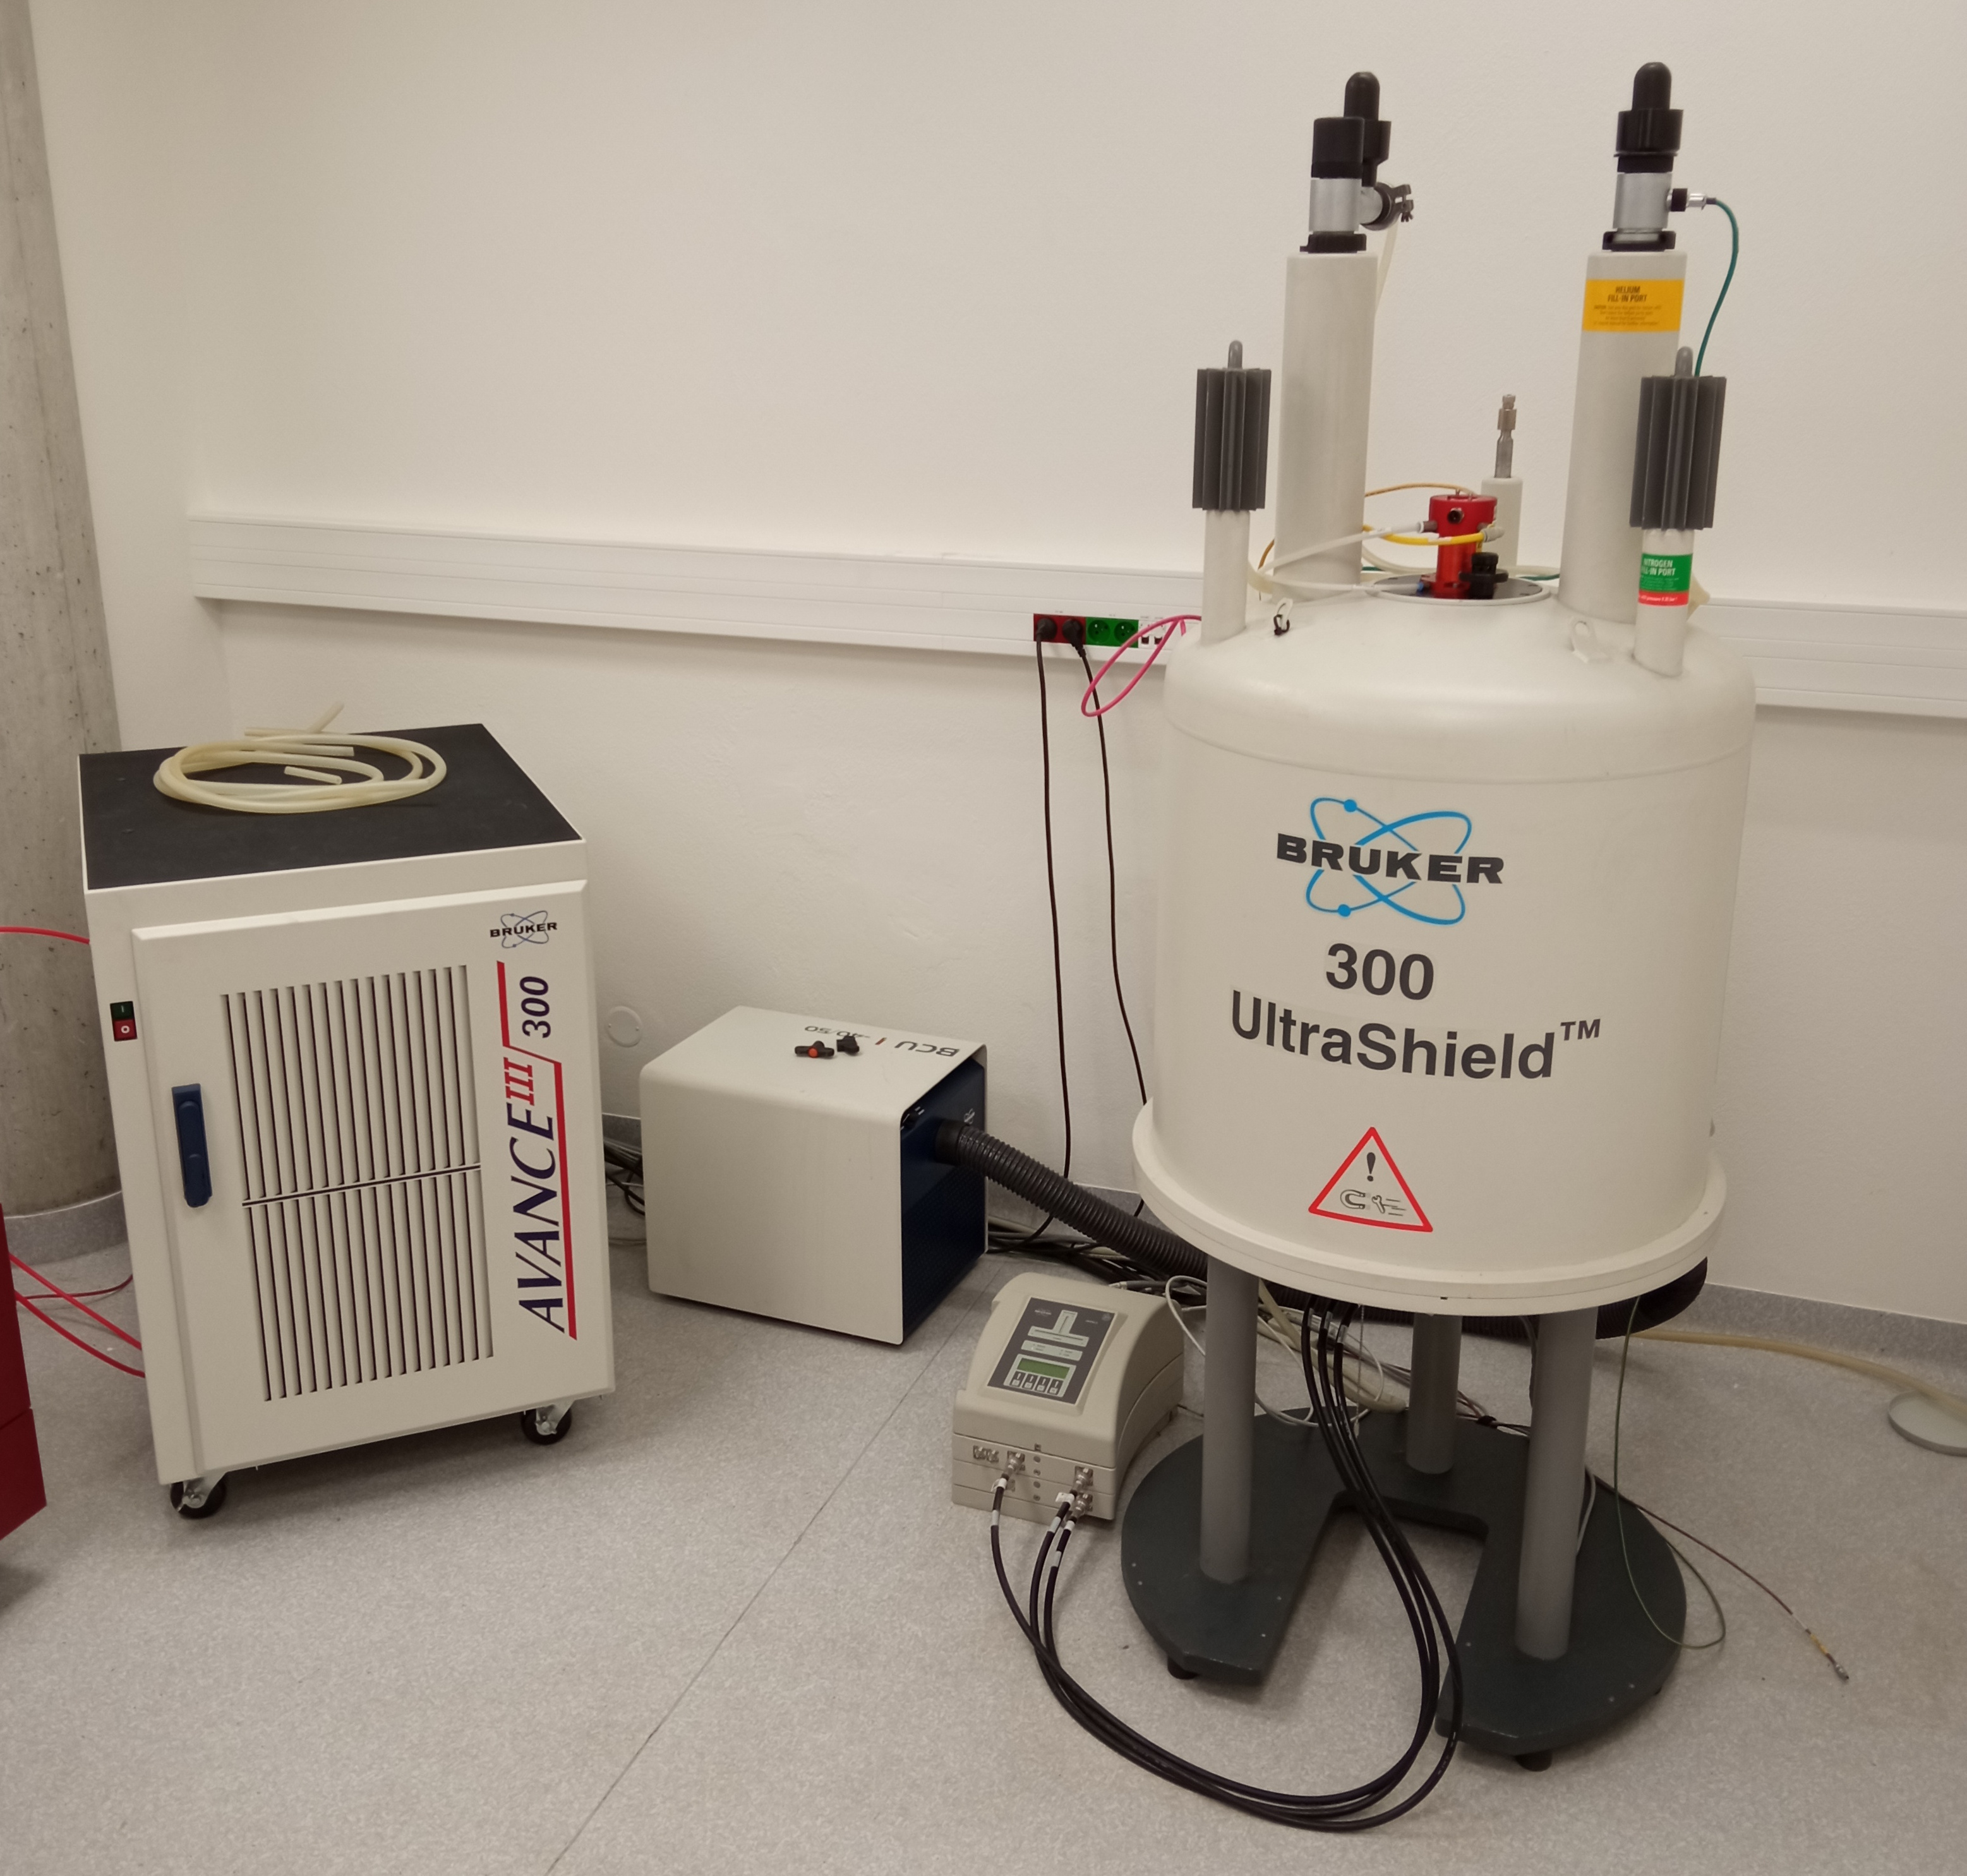
\includegraphics[keepaspectratio,height=6cm]{img/NMR300-1S12.jpg}
	\end{center}

\subsection{Kyselina askorbová}

Prvním úkolem bude naměření $^1$H, $^{13}$C a $^1$H--$^1$H COSY NMR vzorku kyseliny askorbové rozpuštěné v \ce{D2O} a DMSO-d$_6$. Na spektrech si ukážeme vliv rozpouštědla a síly magnetického pole na vzhled spektra.
	\begin{center}
	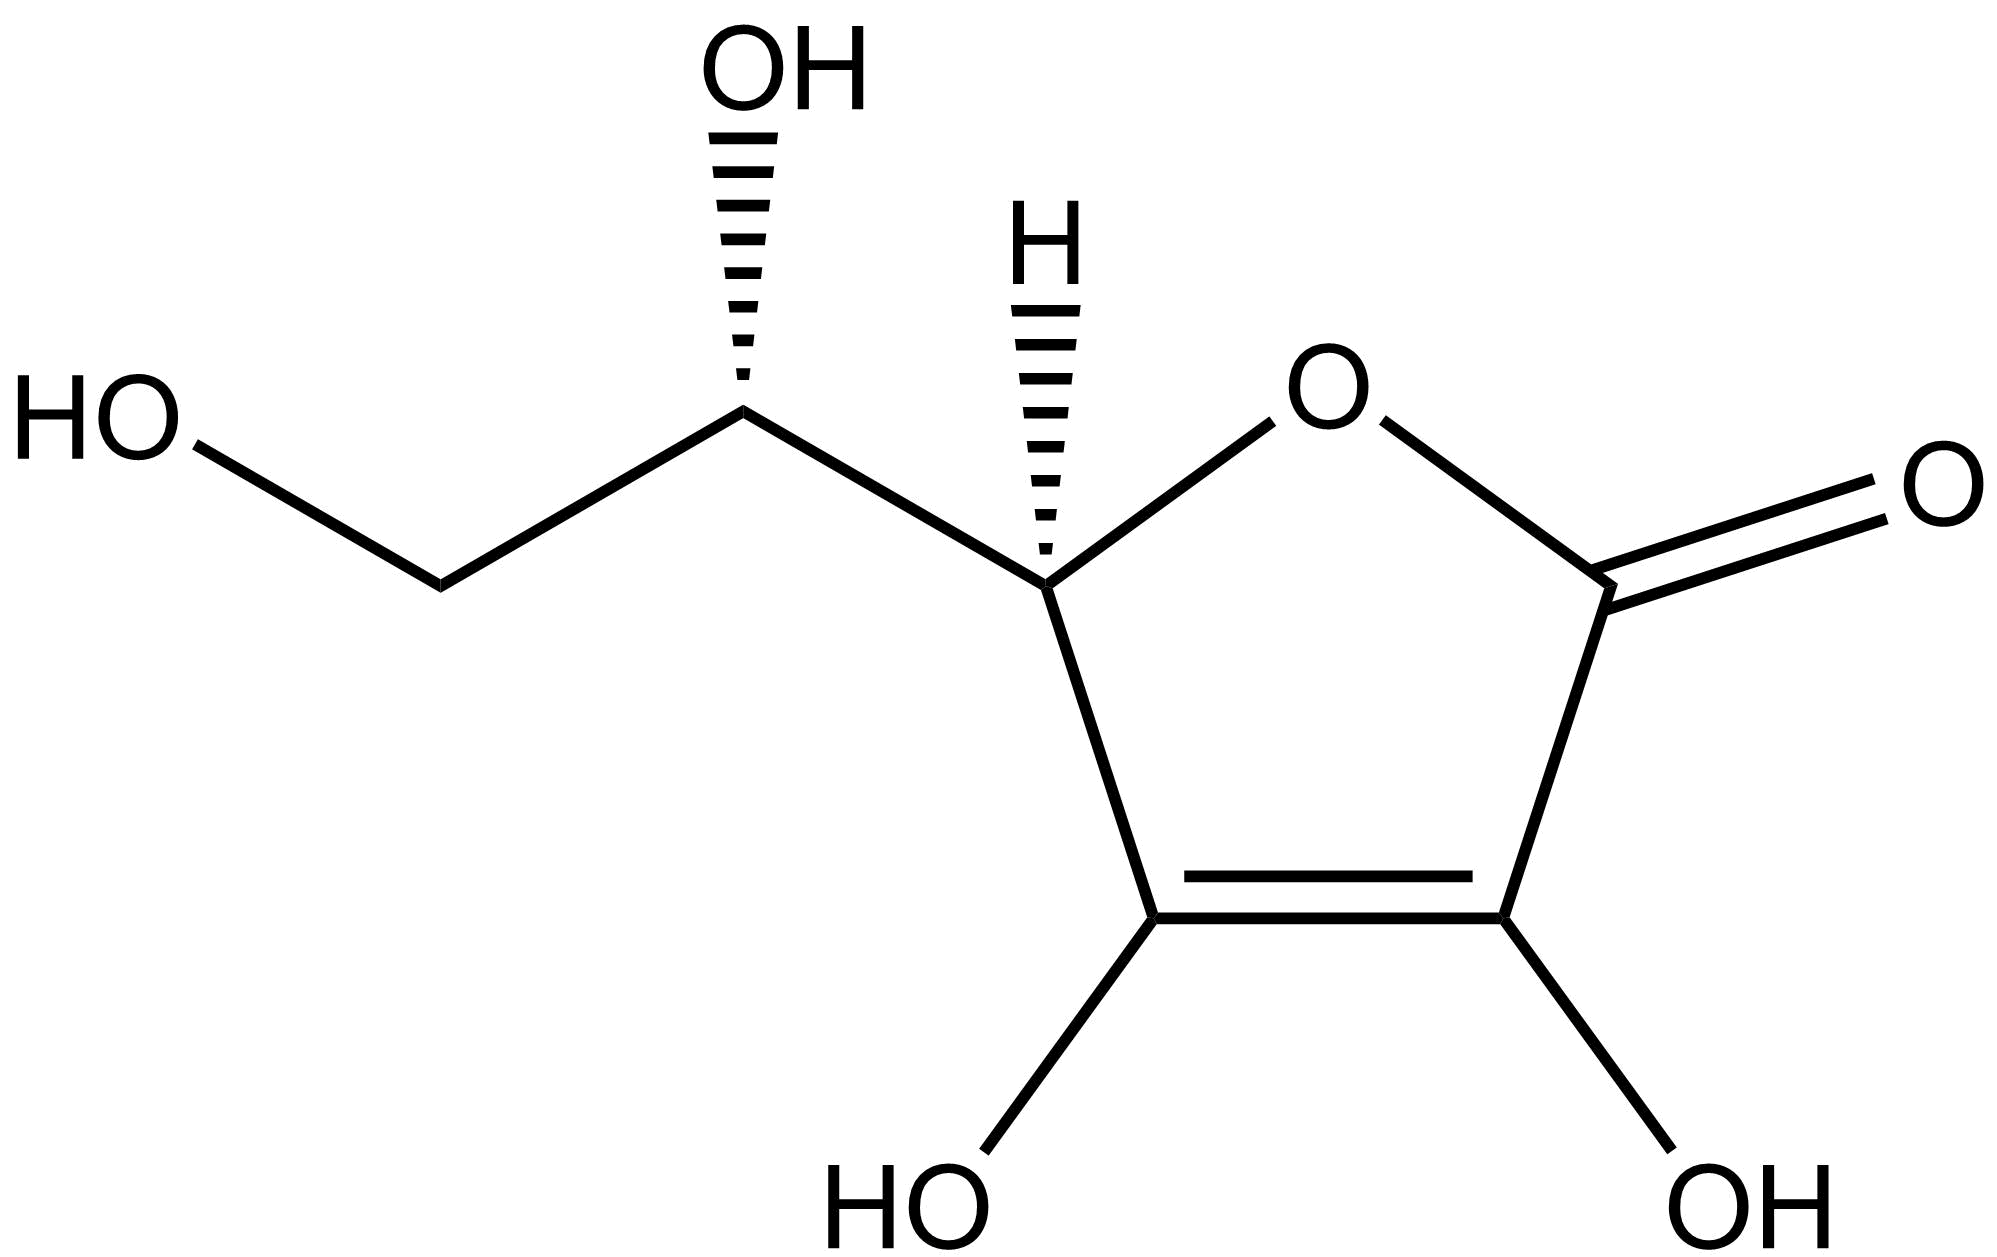
\includegraphics[keepaspectratio,height=5cm]{img/kys-askorbova.png}
\end{center}
\newpage
\subsection{Interakce rozpouštědel}

Pomocí NMR můžeme pozorovat i interakce mezi jednotlivými rozpouštědly. To lze pěkně ilustrovat na směsi toluenu a chloroformu. Během cvičení změříme následujících pět vzorků.
\\

\begin{tabular}{|l|l|l|l|}
	\hline
	\textbf{V$_{Tol}$ [cm$^3$]} & \textbf{V$_{CHCl3}$ [cm$^3$]} & \textbf{$\delta_{CH3}$} 
	& \textbf{$\delta_{CHCl3}$} \\\hline
	0,5 & 0 & & \\\hline
	0,5 & 0,2 & & \\\hline
	0,5 & 0,4 & & \\\hline
	0,5 & 0,6 & & \\\hline
	0,5 & 0,8 & & \\\hline
\end{tabular}

\subsection{Vyhodnocení}

Do protokolu vložte naměřená spektra kyseliny askorbové a interpretujte je. 

Z naměřených dat v druhé úloze sestrojte křivku závislosti chemického posunu na koncentraci chloroformu v toluenu a proložte ji vhodnou křivkou. Vypočítejte rovnici regresní křivky.

\end{document}
